%% For distribution of the original source see the terms
%% for copying and modification in the file samples.dtx.
%% 
%% This generated file may be distributed as long as the
%% original source files, as listed above, are part of the
%% same distribution. (The sources need not necessarily be
%% in the same archive or directory.)
%%
%%
%% Commands for TeXCount
%TC:macro \cite [option:text,text]
%TC:macro \citep [option:text,text]
%TC:macro \citet [option:text,text]
%TC:envir table 0 1
%TC:envir table* 0 1
%TC:envir tabular [ignore] word
%TC:envir displaymath 0 word
%TC:envir math 0 word
%TC:envir comment 0 0
%%
%%
%% For submission and review of your manuscript please change the
%% command to \documentclass[manuscript, screen, review]{acmart}.
%%
%% When submitting camera ready or to TAPS, please change the command
%% to \documentclass[sigconf]{acmart} or whichever template is required
%% for your publication.
%%
%%
\documentclass[acmsmall, review, screen]{acmart}

%%
%% \BibTeX command to typeset BibTeX logo in the docs
\AtBeginDocument{%
  \providecommand\BibTeX{{%
    Bib\TeX}}}

%% Rights management information.  This information is sent to you
%% when you complete the rights form.  These commands have SAMPLE
%% values in them; it is your responsibility as an author to replace
%% the commands and values with those provided to you when you
%% complete the rights form.
\setcopyright{acmcopyright}
\copyrightyear{2022}
\acmYear{2022}
\acmDOI{XXXXXXX.XXXXXXX}

%% These commands are for a PROCEEDINGS abstract or paper.
\acmConference[Conference acronym 'XX]{Make sure to enter the correct
  conference title from your rights confirmation emai}{June 03--05,
  2018}{Woodstock, NY}
%%
%%  Uncomment \acmBooktitle if the title of the proceedings is different
%%  from ``Proceedings of ...''!
%%
%%\acmBooktitle{Woodstock '18: ACM Symposium on Neural Gaze Detection,
%%  June 03--05, 2018, Woodstock, NY}
\acmPrice{15.00}
\acmISBN{978-1-4503-XXXX-X/18/06}


%%
%% Submission ID.
%% Use this when submitting an article to a sponsored event. You'll
%% receive a unique submission ID from the organizers
%% of the event, and this ID should be used as the parameter to this command.
%%\acmSubmissionID{123-A56-BU3}

%%
%% For managing citations, it is recommended to use bibliography
%% files in BibTeX format.
%%
%% You can then either use BibTeX with the ACM-Reference-Format style,
%% or BibLaTeX with the acmnumeric or acmauthoryear sytles, that include
%% support for advanced citation of software artefact from the
%% biblatex-software package, also separately available on CTAN.
%%
%% Look at the sample-*-biblatex.tex files for templates showcasing
%% the biblatex styles.
%%

%%
%% The majority of ACM publications use numbered citations and
%% references.  The command \citestyle{authoryear} switches to the
%% "author year" style.
%%
%% If you are preparing content for an event
%% sponsored by ACM SIGGRAPH, you must use the "author year" style of
%% citations and references.
%% Uncommenting
%% the next command will enable that style.
%%\citestyle{acmauthoryear}

%% Packages
\usepackage{xcolor}
\usepackage{color}
\usepackage{listings}

%% Custom Definitions
\graphicspath{{graph/}}
\definecolor{ForestGreen}{HTML}{009B55}

\lstset{inputpath=code_examples/lib/Examples}
\lstset{
  frame=none,
  xleftmargin=2pt,
  stepnumber=1,
  numbers=left,
  numbersep=5pt,
  numberstyle=\ttfamily\tiny\color[gray]{0.3},
  belowcaptionskip=\bigskipamount,
  escapeinside={*'}{'*},
  language=haskell,
  tabsize=2,
  emphstyle={\bf},
  commentstyle=\color{ForestGreen},
  stringstyle=\mdseries\rmfamily,
  showspaces=false,
  keywordstyle=\bfseries\rmfamily,
  columns=flexible,
  basicstyle=\small\sffamily,
  showstringspaces=false,
  morecomment=[l]\%,
}

%% CUSTOM PACKAGES - NON-ACCEPTED
\usepackage{todonotes}

%%
%% end of the preamble, start of the body of the document source.
\begin{document}

%%
%% The "title" command has an optional parameter,
%% allowing the author to define a "short title" to be used in page headers.
\title{LayeredTypes}
%TODO: Proper Title
%\title[LayeredTypes]{Layered Types -- A structured approach to arbitrarily combine Liquid Types}

%%
%% The "author" command and its associated commands are used to define
%% the authors and their affiliations.
%% Of note is the shared affiliation of the first two authors, and the
%% "authornote" and "authornotemark" commands
%% used to denote shared contribution to the research.
\author{Lukas Abelt}
\email{l.abelt@luabelt.de}
\orcid{1234-5678-9012}
\affiliation{%
  \institution{LASIGE}
  \streetaddress{XXX}
  \city{Lisbon}
  \state{}
  \country{Portugal}
  \postcode{}
}

%%
%% By default, the full list of authors will be used in the page
%% headers. Often, this list is too long, and will overlap
%% other information printed in the page headers. This command allows
%% the author to define a more concise list
%% of authors' names for this purpose.

%%
%% The abstract is a short summary of the work to be presented in the
%% article.
\begin{abstract}
	\todo[inline]{TODO: Abstract}
\end{abstract}

%%
%% The code below is generated by the tool at http://dl.acm.org/ccs.cfm.
%% Please copy and paste the code instead of the example below.
%% TODO
\begin{CCSXML}
<ccs2012>
 <concept>
  <concept_id>10010520.10010553.10010562</concept_id>
  <concept_desc>Computer systems organization~Embedded systems</concept_desc>
  <concept_significance>500</concept_significance>
 </concept>
 <concept>
  <concept_id>10010520.10010575.10010755</concept_id>
  <concept_desc>Computer systems organization~Redundancy</concept_desc>
  <concept_significance>300</concept_significance>
 </concept>
 <concept>
  <concept_id>10010520.10010553.10010554</concept_id>
  <concept_desc>Computer systems organization~Robotics</concept_desc>
  <concept_significance>100</concept_significance>
 </concept>
 <concept>
  <concept_id>10003033.10003083.10003095</concept_id>
  <concept_desc>Networks~Network reliability</concept_desc>
  <concept_significance>100</concept_significance>
 </concept>
</ccs2012>
\end{CCSXML}
%TODO
%\ccsdesc[500]{Computer systems organization~Embedded systems}
%\ccsdesc[300]{Computer systems organization~Redundancy}
%\ccsdesc{Computer systems organization~Robotics}
%\ccsdesc[100]{Networks~Network reliability}

%%
%% Keywords. The author(s) should pick words that accurately describe
%% the work being presented. Separate the keywords with commas.
%TODO: Keywords
\keywords{}
%% A "teaser" image appears between the author and affiliation
%% information and the body of the document, and typically spans the
%% page.
\begin{teaserfigure}
  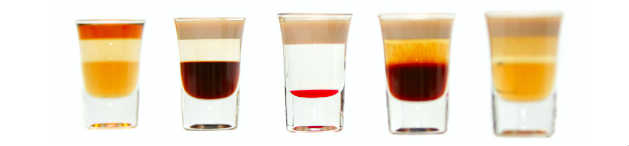
\includegraphics[width=\textwidth]{layered-shots.jpg}
  \label{fig:teaser}
  \caption{Layers in Liquids}
\end{teaserfigure}

\received{20 February 2007}
\received[revised]{12 March 2009}
\received[accepted]{5 June 2009}

%%
%% This command processes the author and affiliation and title
%% information and builds the first part of the formatted document.
\maketitle

\section{Introduction}
\subsection{Context}
Modern program languages such as C++, Haskell, Rust or Java use type systems to ensure certain promises about the correct behavior of an implementation. In essence, the type system allows the programer to specify what inputs to accept for a program or function and what outputs it will produce. While these guarantees already prevent a multitude of runtime errors, they alone cannot prevent e.g. divisions by yero or out of range accesses in arrays.

One approach to bridge this gap is the introduction of \textit{Refinement Types}, also referred to as \textit{Liquid Types}. These allow us to annotate the traditional type system with additional logical predicates in order to ensure semantic properties, which can be checked statically at compile time. Using these techniques also allows us to define pre- and post-conditions on functions' arguments and return values. By properly defining these contracts a developer can clearly communicate and moreover enforce how other developers' code is allowed to interface with their implementations. Examples for constraints might include any of the following:

\begin{itemize}
	\item Ensuring values are in certain bounds
	\item Ensuring that a list is non-empty
	\item Ensuring that data structures certain to specific semantic properties e.g. that they are sorted
\end{itemize}

All in all, refinement types are valuable building blocks to creating reliable software systems. Using them can minimize the risk of any unhandled run-time errors occuring which might lead to undesired or even undefined behavior.

\subsection{Motivation}

While Refinement Types already vastly imrpove traditional type systems, current implementations still expose some drawbacks in their practical usage. One of these challenges stems from the fact that during the static analysis, each refinement is treated as a single monolithic requirement that needs to be fulfilled. However in reality, a refinement might combine different properties of a type that may benefit from being treated individually.

One example for such a refinement in LiquidHaskell is shown in \ref{lst:combined_lt}. There, we define a function that extracts the maximum value of a (descendingly) ordered, non-empty list. In this example, this operation is equivalent to simply extracting the \texttt{head} of a list. While we only define one refinement, it actually operates on two different properties of a list. First, it imposes a restriction on it's \texttt{size} by requiring it to be non-empty, while the second restriction imposes an order on the list elements.

\lstinputlisting[firstline=6,caption={Example for a function with a combined Refinement Type in LiquidHaskell},label={lst:combined_lt}]{CombinedLT.hs}

While the refinement concerns two different aspects of the list that are independent from each other, current static analysis implementations of Liquid Types will treat it only as a single combined requirement to be fulfilled. However especially developers could benefit from a system that treats them independently: When writing code that interfaces with already existing codes such a separated approach may give a developer more fine-grained information on which requirements they still need to fulfill in their implementation.

Effectively one could treat such different requirements as separate \textit{Layers} that can be verified independently. Additionally with a proper implementation using such layers may also result in an implementation benefit, that different Layers can be defined individually and combined arbitrarily, as opposed to the example in Listing \ref{lst:combined_lt} where the combination of the two traits had to be explicitly defined as an refinement on it's own.

One other possible usage of such an iterative approach is that it could allow to more flexibly add different static analysis approaches on top of each other. For example \ref{handley2020} have shown how to use liquid types in Haskell to statically perform cost analysis of different resources such as memory consumption or computational complexity. In their approach they showed that liquid types can be used to reason about their upper and lower bounds. However, in their work they only analysed one resource at a time. However, using a layered approach would allow to easily combine these different resource analyses to eg. track and reason about both memory usage and computational complexity.

\subsection{Problem Definition}

Current Liquid Type implementations limit us to only defining one liquid type for variables, arguments or return types. This forces us to combine all properties we want to statically check and verify into one big predicate. Using such an approach has the drawback that all properties are checked simultaneously which might make it difficult for a developer to identify due to which property a type error occurs. Additionally previously declared liquid types may not be reused when wanting to refine them further.

We therefore propose an implementation of \textit{Layered Liquid\todo{Just Layered or Layered Liquid?} Types}, that allows to define types as a conjunction of previously defined Liquid Types. These types are then checked iteratively to ensure compability between functions and arguments.

Assume we have a function \texttt{f} that takes as input a single liquid type $T^{in}$ refined by the predicates $p^{in}_1,\cdots,p^{in}_n$ and result type \texttt{out} and a variable \texttt{arg} of liquid type $T^{arg}$ refined by the predicates $p^{arg}_1,\cdots,p^{arg}_m$:

\begin{lstlisting}[mathescape=true]
	-- Liquid Type Definitions
	{-@ type $T^{in}$ t = { t | $p^{in}_1 \wedge ... \wedge p^{in}_n$  } @-}
	{-@ type $T^{arg}$ t = { t | $p^{arg}_1 \wedge ... \wedge p^{arg}_m$ } @-}

	f : $T^{in}$ -> out 
	arg : $T^{arg}$
\end{lstlisting}


When now calling \texttt{f} with \texttt{arg} as an argument, current implementations of liquid types will check for compability of the arguments in a manner similar to:

$$ \left( \bigwedge^{m}_{i=1} p^{arg}_i \right) \implies \left( \bigwedge^{n}_{j=1} p^{in}_j \right) $$

In our layered approach we rather propose that we can define separate layered types for each predicate and easily use their conjunction as the specific refined type for arguments and values:

\begin{lstlisting}[mathescape=true]
	-- Liquid Type Definitions for inputs to f
	{-@ type $T^{in}_1$ t = { t | $p^{in}_1$ } @-}
	{-@ type ... @-}
	{-@ type $T^{in}_n$ t = { t | $p^{in}_n$ } @-}

	-- Liquid Type Definitions for arg
	{-@ type $T^{arg}_1$ t = { t | $p^{arg}_1$ } @-}
	{-@ type ...  @-}
	{-@ type $T^{arg}_m$ t = { t | $p^{arg}_m$ } @-}

	f : {$T^{in}_1 \wedge ... \wedge T^{in}_n$} -> out 
	arg : {$T^{arg}_1 \wedge ... \wedge T^{arg}_m$}
\end{lstlisting}


In this layered approach predicates are not checked simultaneously but rather in an iterative way, which could intuitively rather be expressed as the (which is semantically equivalent to the version above):

$$ \bigwedge^{n}_{j=1} \left( \bigwedge^{m}_{i=1} p^{arg}_i \implies  p^{in}_j \right) $$

While on first glance this approach could be described as an approach to \textit{Gradual Verification}, we will explicitly refer to our approach as \textit{Layered} to distinguish it from \textit{Gradual Verification} techniques. While the latter deal with the gradient between incomplete and complete information (in that case on types), our approach is rather concerned not with what information is available on the typing but rather how it is processed. While gradual approaches might still type-check with incomplete typing information our approach would fail to typecheck in such a scenario as it still requires complete information. 

\subsection{Impact}

We expect our approach to have the following impacts on Liquid Types in practice:

\paragraph{Improved Error Messages}

One current challenge when using liquid types is that all predicates for a type are checked simultaneously. This can make it difficult to identify which predicate caused a type liquid error. By separating the predicates into separate \textit{Layers} and verifying them individually, it is possible to precisely identify the predicate causing the type error. We expect this to help developers to more easily identify and fix these type errors in their code.

\paragraph{Improved Usability and Reusability}

In current Liquid Type implementations, types that require multiple predicates are defined as a single type. This may make it difficult for a developer to directly identify which properties a specific liquid type ensures. By separating different properties into a more fine-grained layered approach, this may make it easier to identify these properties. Additionally, by separating the predicates into different layers, it is possible to reuse previously defined liquid types in a more flexible way. For example, if a developer wants to refine a previously defined liquid type, they can now do so by adding a new layer to it, instead of having to redefine the entire type.

\paragraph{Improved Composability}

In addition to the improved reusability of our approach, we also expect it to improve the composability of different liquid types. With our suggested approach, new refinements can simply be created by composing already existing layers. This vastly increases modularity of the liquid type approach. It also may allow to re-use layers that have already been defined by other developers for ones own implementation.

\subsection{Approach}
We will start by giving a brief overview of the general principles of refinement types and liquid types in general in section \ref{sec:background}. Additionally, we will discuss the current state of the art in liquid types and gradual verification in section \ref{sec:related}. 

In section \ref{sec:implementation} we will first give a more detailed description of our approach and define a simple functional language that we will use for further demonstration. We will then implement a prototype type checker for our layered approach. Using this simple prototype we will showcase how our approach can be used on various simple examples.

In section \ref{sec:evaluation} we will discuss the limitations of our approach and possible extensions. Additionally, we will evaluate how our approach compares to using a pure, non-layered, verification approach.

Test

\subsection{Contributions}
\section{Background}
\label{sec:background}
\section{Related Work}
\label{sec:related}
\section{Implementation}
\label{sec:implementation}

In this section we will describe our implementation of a layered typing approach in detail. We will start by describing the simple functional language we will use for our examples. We will then describe how our layered type checker is implemented. Finally, we will showcase how our approach can be used on various simple examples.

\subsection{Language}
\label{ssec:language}

To demonstrate our layered approach we implemented a simple functional language. The syntax of said language is described in \ref{fig:lang}. The language is similar to most simple functional languages and generally follows the reduction semantics of a standard Hindley-Milner type system. The only data types available in the language are the \texttt{Int} and the \texttt{Bool} type. However, the language does not strictly require the programmer to explicitly specify the type of a variable.

\begin{figure}[ht!]
\begin{align*}
	id \in \texttt{Ident}\ 	&::=\ [a...zA...Z]+ \\
	v \in \texttt{Var}\ 	&::=\ id \\
	f \in \texttt{Fun}\ 	&::=\ id_1\ id_2\ \{\ s\ \}\\
	e \in \texttt{Expr}\ 	&::=\ v\ |\ (\ e\ \circledplus\ e\ )\ |\ (e\ \circleddot\ e)\ |\ c \\
	c \in \texttt{Const}\ 	&::=\ \texttt{True}\ |\ \texttt{False}\ |\ \mathbb{Z} \\
	s \in \texttt{Stmt}\ 	&::=\ v\ :=\ e\ |\ f(v)\ |\ \texttt{if}\ v\ \texttt{then}\ s\ \texttt{else}\ s\ |\ \texttt{let}\ v\ :=\ e\ \texttt{in}\ s\ |\ l \\
	l \in \texttt{Layer}\ 	&::=\ id_1::id_2::\texttt{String} \\
	\circledplus\ 		&::=\ \texttt{+}\ |\ \texttt{-} \\
	\circleddot\ 		&::=\ \texttt{!=}\ |\ \texttt{==}\ |\ \texttt{<} \ |\ \texttt{>} \ |\ \texttt{<=} \ |\ \texttt{>=} \\
\end{align*}
\caption{Syntax of the simple functional language}
\label{fig:lang}
\end{figure}

Additionally to standard operations, the syntax of the language supports creating layers that can be applied onto each identifier. The syntax of a layer consists of the following:
\begin{itemize}
	\item $id_1$ -- The name of the identifier to be refined
	\item $id_2$ -- The name of the layer
	\item An arbitrary \textit{String} that represents the refinement. Note that the syntax does not restrict the format of this string, as this information will be parsed later by the corresponding type checking layer.
\end{itemize}

These layers can then be used to refine an identifier. In a very basic and minimal approach these layers can be used to annotate types to variables and identifiers. Additionally, one might add additional layers to a variable to ensure more properties. Each layer will be checked individually and independently. A more detailled approach of the architecture behind our layered approach will be described in section \ref{ssec:architecture}.

An example of a program written in our language can be seen in \ref{lst:fac_example}. The program defines a factorial function that is refined in two layers. The first layer \textit{base} is a simple type layer that defines that \texttt{fac} takes an \texttt{Int} and returns an \texttt{Int}. The second layer \textit{liquid} is a refinement layer that refines that the input should be greater or equal to zero and that the output will be greater than zero.

\begin{lstlisting}[caption={Example of a factorial function in our simple language}, label={lst:fac_example}]
fac::base:: Int -> Int
fac::liquid:: {v:Int | v >= 0} -> {v:Int | v > 0}
fac x { 
let cond := (x == 0) in
	if cond then 
		1 
	else 
		x * fac (x - 1) 
}
\end{lstlisting}

\begin{table}[h!]
  \begin{center}
    \begin{tabular}{cl} 
      \\
      \(\frac
         {x \ : \ \sigma \ \in \ \Gamma}
        {\Gamma \  \vdash \ x \ : \ \sigma} \) 
      &  [\texttt{Var}]  \\
      \\
      
      \\
      \(\frac
        {\Gamma \  \vdash \ {e}_{0} \ : \ \tau \rightarrow {\tau}' \;\;\;\; \Gamma \  \vdash \  {e}_{1} \ : \ \tau}
        {\Gamma \vdash {e}_{0} \; {e}_{1} \ : \ {\tau}'} \)
      & [\texttt{App}] \\
      \\
      
      \\
      \(\frac
        {\Gamma , \ x \ : \ \tau \ \vdash \ e \ : \ {\tau}'}
        {\Gamma \ \vdash \ \lambda x \ . \ e \ : \ \tau \rightarrow{\tau}'}\)
      & [\texttt{Abs}] \\
      \\
      
      \\
      \(\frac
        {\Gamma \ \vdash \ {e}_{0} \ : \ \sigma \;\;\;\; 
         \Gamma, \ x \ : \ \sigma \ \vdash \ {e}_{1} \ : \ \tau}
        {\Gamma \ \vdash \ \texttt{let} \ x \ = \ {e}_{0} \ \texttt{in} \ {e}_{1} \ : \ \tau}\)
      & [\texttt{Let}] \\ 
      \\
      
      \\
      \(\frac
        {
            \newline
            \Gamma \ \vdash \ e \ : \ {\sigma}' \;\;\;\;
            {\sigma}' \ \sqsubseteq  \ \sigma
        }
        {
            \Gamma \ \vdash \ e \ : \ \sigma
        }\)
      & [\texttt{Inst}] \\
      \\
      
      \\
      \(
       \frac
       {
        \Gamma \ \vdash \ e \ : \ \sigma \;\;\;\;
        \alpha \ \notin \text{free}(\Gamma)
       }
       {
        \Gamma \ \vdash \ e \ : \ \forall \ \alpha \ . \ \sigma
       }
      \)
      & [\texttt{Gen}] \\
      \\
    \end{tabular}
  \end{center}
\end{table}

\subsection{Language Implementation Architecture}
\label{ssec:architecture}

The implementation of our language will be done in the \texttt{Python} programming language. Roughly speaking, the implementation will consist of three parts, which we will describe throughout this section:

\begin{enumerate}
	\item A parser that parses the input program and creates an abstract syntax tree (AST) of the program (\ref{sssec:parser}).
	\item A layered type checker that checks the defined type layers for the tree incrementally (\ref{sssec:layered_type_checker}).
	\item A code generator that generates the corresponding code for the input program (\ref{sssec:code_generator}).
\end{enumerate}

\subsubsection{Parser}
\label{sssec:parser}

\subsubsection{Layered Type Checker}
\label{sssec:layered_type_checker}

\subsubsection{Code Generator}
\label{sssec:code_generator}

\subsection{Examples}
\label{ssec:examples}

\section{Evaluation}
\label{sec:evaluation}
\section{Conclusion}
\label{sec:conclusion}
\section{Acknowledgments}
\label{sec:acknowledgments}

\end{document}
\endinput
%%
%% End of file `sample-acmsmall-conf.tex'.
